\documentclass[11pt]{article}
\usepackage[top=2cm, bottom=3cm, left=2cm, right=2cm]{geometry}
%\renewcommand{\thesubsubsection}{\thesubsection.\roman{subsubsection}}
\usepackage{subfiles}
\usepackage{gensymb}
\usepackage{amsmath}
\usepackage{units}
\usepackage{amssymb}
\usepackage[numbers]{natbib} % use this if not all your bibitems have an author and a year
%\usepackage{natbib}
\usepackage{hyperref}
\usepackage{color}
\usepackage[toc,page]{appendix}
\usepackage[printonlyused]{acronym}
\usepackage{multicol}
%%%%%%%%%%%%%%%%%%%%%%%%%%%%%%%%%
\DeclareRobustCommand\nocite[1]{%
    {\def\cite##1{\ignorespaces}#1}}
\newcommand\nocitecaption[1]{\caption[\nocite{#1}]{#1}}

%\nocitecaption{\caption this is my caption[\nocite{}]{}}

%%%%%%%%%%%%%%%%%%%%%%%%%%%%
\newcommand{\code}{\texttt}

% you need this to input images in the way used in the results (copy paste that layout wherever you want and just change the image file name, the caption and the label
\usepackage{graphicx}
\usepackage[numbered, framed]{mcode}
\usepackage{float}
\usepackage{lscape}

% following lines make sure that tables and figures are labelled as Figure Ch.Num
\usepackage{chngcntr}
\counterwithin{table}{section}
\counterwithin{figure}{section}

%setting up page headers/footers
\usepackage{fancyhdr}
\setlength{\headheight}{25pt} 
\usepackage{lastpage}
\pagestyle{fancy}
\fancyhf{}

%for fitting tables to a page
\usepackage{tabularx}

%for aligning images side by side
\usepackage{subcaption}
\usepackage{graphicx}

%\lhead{Technical Report}
\rhead{ASP Labs - 6562233}
\lfoot{EEEM007: Advanced Signal Processing}

%format for code listings
\usepackage{listings}
\lstset{
	basicstyle=\ttfamily,
	columns=fullflexible,
	frame=single,
	breaklines=true,
	postbreak=\mbox{\textcolor{red}{$\hookrightarrow$}\space},
}

% THIS IS A COMMENT WE CAN WRITE WHATEVER WE WANT HERE WITHOUT IT SHOWING UP ON THE FINAL DOCUMENT

%Note for Kausthub: be careful on the difference between \input and \include. Can nest inputs. Can't nest includes. can't include within an input. can input under and include or another input. include forces pagebreak

%FOR TABLES:: Write in Excel then use this website
%http://www.tablesgenerator.com/

% Removes indents from new paragraphs
\setlength{\parindent}{0pt}

\begin{document}
	\pagenumbering{gobble}		%holds page numbering so that it doesn't start yet
	
    \input{./AssignmentCoversheet.tex}
%	\tableofcontents

\pagebreak
%\listoffigures
%\listoftables
    \acresetall
    %starts numbering pages from here and adds it to the right footer
	\pagebreak
	\rfoot{\thepage}
	\rhead{\nouppercase{\rightmark}}
	\pagenumbering{arabic}
    
    % Contents goes here
    \section{Introduction}\label{s:intro}
This report includes the documentation of a number of experiments carried out as stipulated by the handout provided. The six experiments attempted will explore the effect of the following variables on a pattern recognition system.

\begin{enumerate}
	\item The effect of training sample size on classifier performance.
	\item The effect of test set size on classifier performance, as well as dimensionality effects.
	\item The effect of the size of test set on the reliability of the empirical error count estimator.
	\item To explore the relationship between class separability and error probability.
	\item The effect, on the classifier error probability, of discrepancies between the true and assumed class probability distribution models.
	\item Comparing kNN with a Gaussian classifier.
\end{enumerate}

Experiments 1-4 and 6 will each be presented in the following sections, and though some attempt was made at Experiment 5, only a partial solution will be presented in this report.

%
%\begin{figure}[H]
%	\centering
%	\includegraphics[width=.6\linewidth]{./img/ann_nielsen.png}
%	\caption{Shallow Network Architecture \cite{Nielsen2015}}
%	\label{fig:ann}
%\end{figure}

    \section{Experiment 1}

write a description of the experiment

write a prediction about the outcomes based off theory

\begin{figure}[H]
        \centering
        \begin{subfigure}[b]{0.475\textwidth}
            \centering
            \includegraphics[width=\textwidth]{./code/Exp1-results/10iters/Train10.png}
            \caption[]%
            {{\small 10 sample training set}}    
            \label{fig:train10}
        \end{subfigure}
        \hfill
        \begin{subfigure}[b]{0.475\textwidth}  
            \centering 
            \includegraphics[width=\textwidth]{./code/Exp1-results/10iters/Train50.png}
            \caption[]%
            {{\small 50 sample training set}}    
            \label{fig:train50}
        \end{subfigure}
        \vskip\baselineskip
        \begin{subfigure}[b]{0.475\textwidth}   
            \centering 
            \includegraphics[width=\textwidth]{./code/Exp1-results/10iters/Train100.png}
            \caption[]%
            {{\small 100 sample training set}}    
            \label{fig:train100}
        \end{subfigure}
        \quad
        \begin{subfigure}[b]{0.475\textwidth}   
            \centering 
            \includegraphics[width=\textwidth]{./code/Exp1-results/10iters/Test100.png}
            \caption[]%
            {{\small 100 sample test set}}    
            \label{fig:test100}
        \end{subfigure}
        \caption[ ]
        {\small Visualisation of examples of test and training data generated for Experiment 1.} 
        \label{fig:SampleDatasets}
    \end{figure}





\subsection{Results}

\begin{figure}[H]
	\centering
	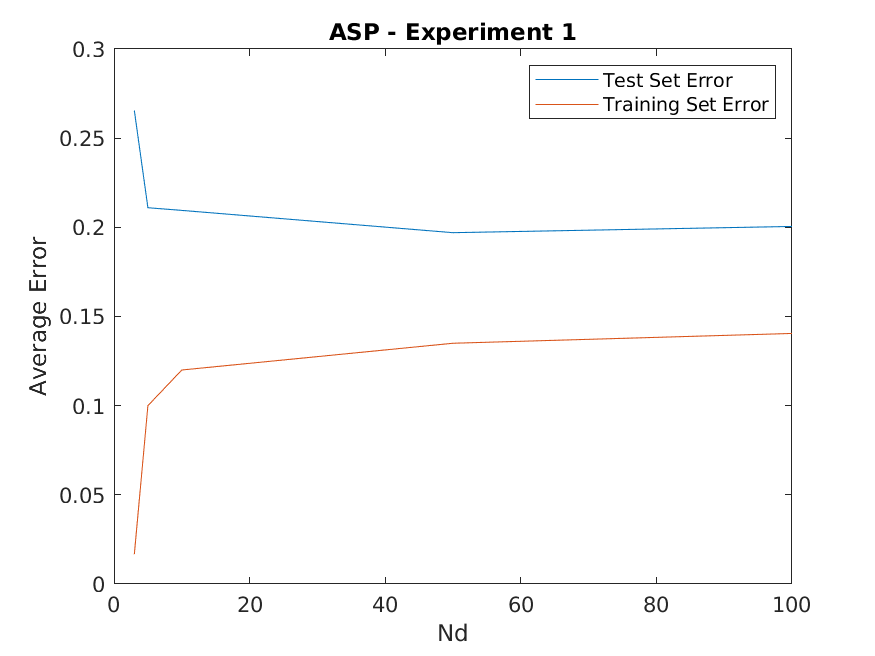
\includegraphics[width=.6\linewidth]{./code/Exp1-results/10iters/ErrorComparison.png}
	\caption{Experiment 1 Results}
	\label{fig:exp1}
\end{figure}


\subsection{Discussion}

    \section{Experiment 2}
This experiment investigates the effects of pattern recognition in higher dimensional domains. In order to do this the training error would now be regenerated for every new dimension considered (5, 10, 15), but would remain constant in that loop. The test dataset, however, would be regenerated on every iteration of the experiment. Once again following a similar format to the training cycle and repetitions as in Experiment 1, this experiment also has one fundamental difference in that since the training error will effectively remain constant (relative to the dimension). However the testing error should approach the true error value which was approximated by the $E(500)$ error probability approximation. As instructed the covariance matrix was selected to be an identity matrix, and the class means were designed in a way that $\mu_{1}$ is a random vector of integers, and that $\mu_{2}$ is offset by a random fractional distance from $\mu_{1}$. The weights were manually adjusted to ensure that the error probability value remained within the range of 5-10\% for all dimensions.

\subsection{Results \& Discussion}
Unlike the expected convergence, the errors were seen to oscillate prior to convergence. This oscillation was more present at lower values of $N_{D}$ and convergence to reasonable performance needed larger training datasets in lower dimensions. As seen in Figure \ref{fig:exp2-a} the oscillation lasts longer in the 5 dimensional space as opposed to the 10 and 15 dimensional spaces as seen in Figure \ref{fig:exp2-b}. Though these experiments were conducted in low granularity it's clear that between 100-200 training sample sets are needed at a higher dimension of 10 or 15. 

\begin{figure}[H]
	\centering
	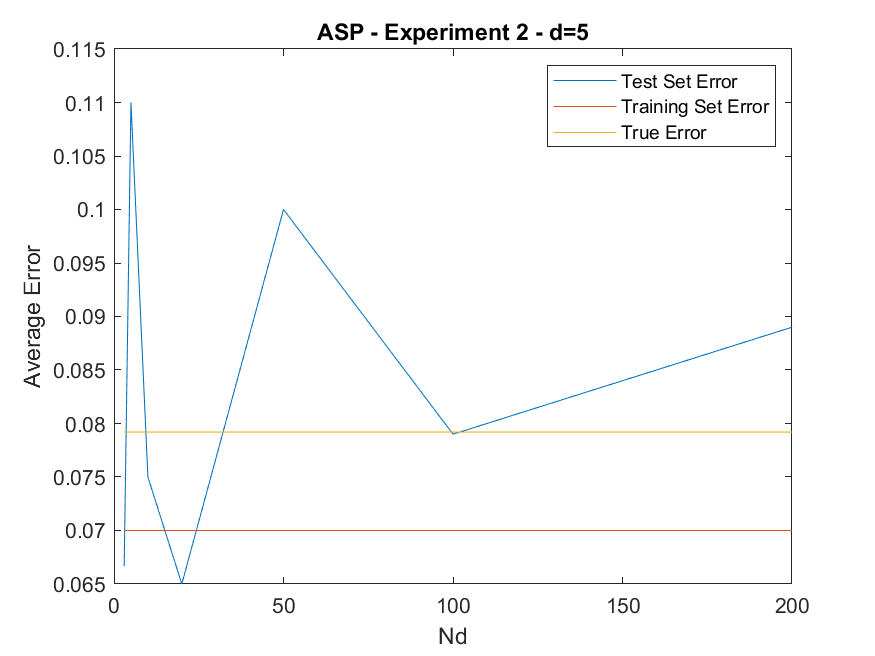
\includegraphics[width=.8\linewidth]{./code/Exp2-results/ErrorComparison_5.png}
	\caption{5 Dimensions}
	\label{fig:exp2-a}
\end{figure}

\begin{figure}[h]
	\centering
	\begin{subfigure}{.5\textwidth}
		\centering
		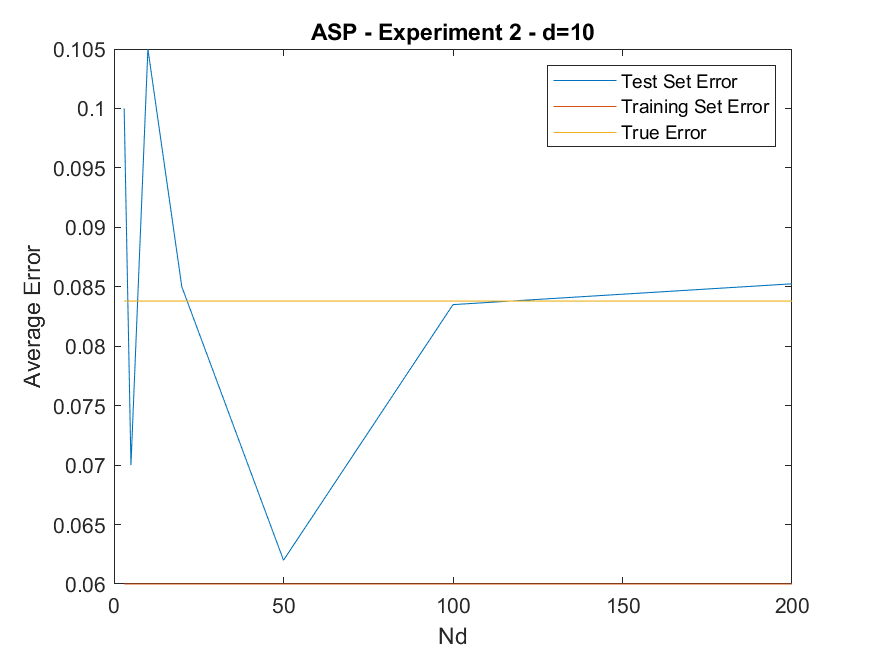
\includegraphics[width=.95\linewidth]{./code/Exp2-results/ErrorComparison_10.png}
		\caption{10 Dimensions}
	\end{subfigure}%
	\begin{subfigure}{.5\textwidth}
		\centering
		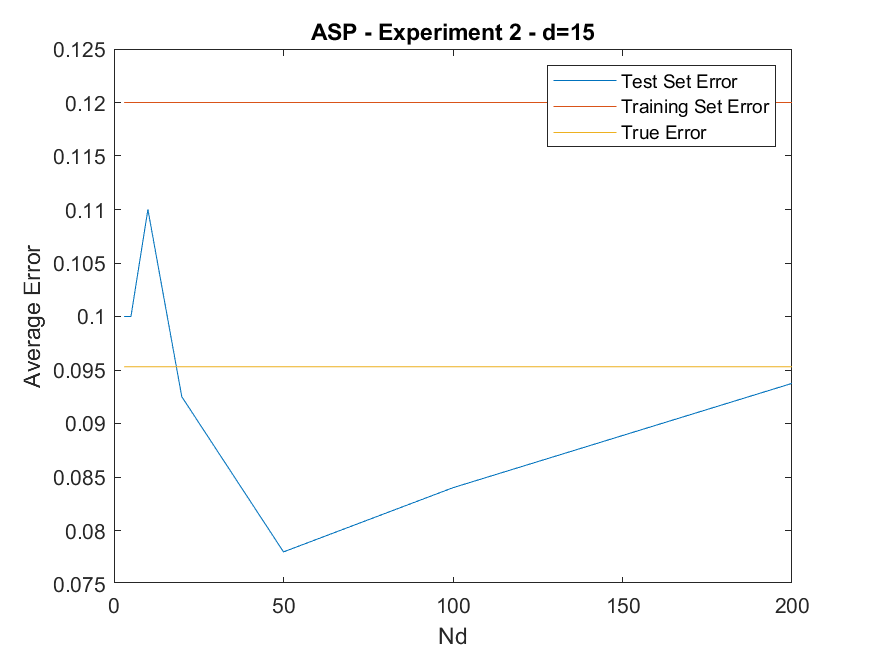
\includegraphics[width=.95\linewidth]{./code/Exp2-results/ErrorComparison_15.png}
		\caption{15 Dimensions}
	\end{subfigure}
	\caption{Experiment 2 Results - Mean Error Comparison vs Test Set Size}
	\label{fig:exp2-b}
\end{figure}

    \pagebreak
\section{Experiment 3}
This experiment investigates the size of the test set and the reliability of a system given greater independence in datasets. This time the class means are defined in a similar manner to the process in Experiment 2, however the weighting differs as the error probability is given a wider allowable range of 1-10\%. Ten such test sets are created and stored independently, and the process once again iterates 10 times for each sample size $N_{D} = 5, 10, 20, 50$ and then intervals of 50 until $N_{D} = 500$. Once again, as in Experiment 2, the Test Set Error should converge to the true error, and the training set error should remain constant as the training set itself is never changed.

\subsection{Results and Discussion}
As expected the error converges to the true error and, as mentioned in Experiment 2, this occurs at $N_{D} > 200$ in the 5-dimensional space selected for this experiment. The oscillatory nature observed previously in Experiment 2 presents similar characteristics here as the standard deviation in error varies as seen in \ref{fig:Exp3}(b). So far this allows us to conclude that greater reliability in approximating the true error can be achieved with larger test data sets. However the standard deviation does not significantly reduce suggesting that an increase in test dataset may not be enough to improve reliability in the system - and that the increase in reliability is more prevalent when an increase in training data is offered (as in Experiment 1).

\begin{figure}[h]
	\centering
	\begin{subfigure}{.5\textwidth}
		\centering
		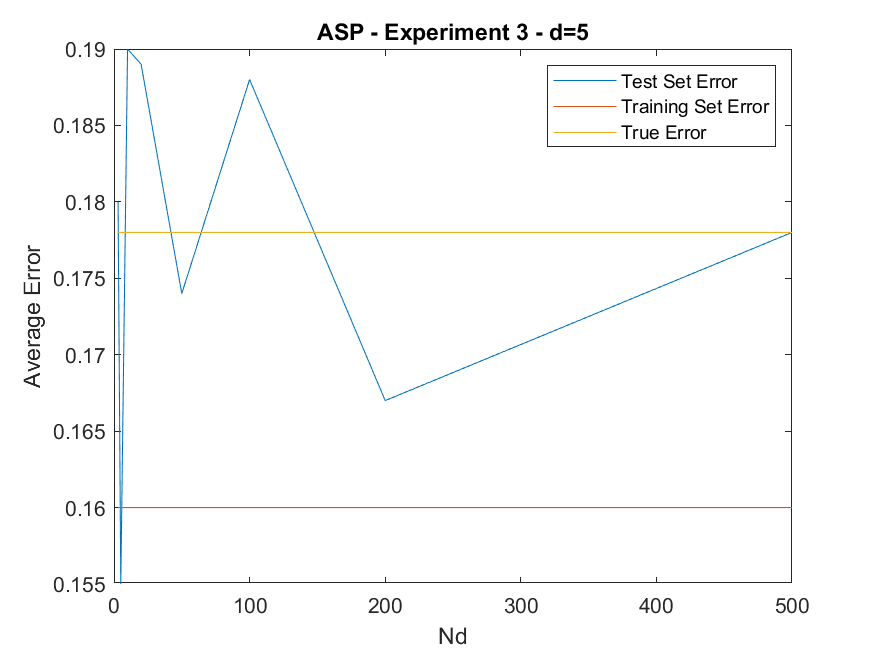
\includegraphics[width=.95\linewidth]{./code/Exp3-results/ErrorComparison_5.png}
		\caption{5 Dimensions}
	\end{subfigure}%
	\begin{subfigure}{.5\textwidth}
		\centering
		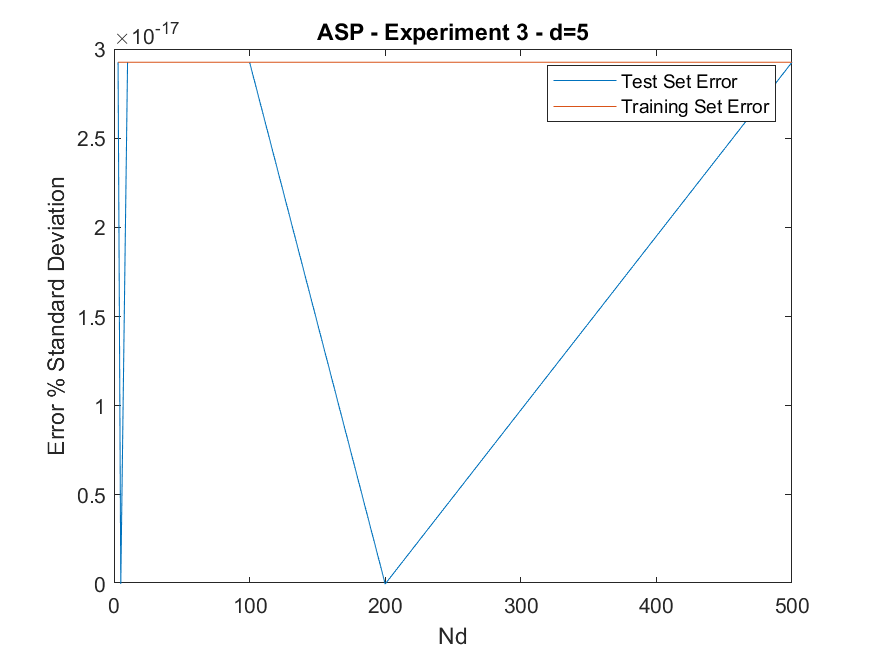
\includegraphics[width=.95\linewidth]{./code/Exp3-results/ErrorStandardDeviation_5.png}
		\caption{Standard Deviation of Error \% vs Test Set Size}
	\end{subfigure}
	\caption{Experiment 3 Results - Test Set Size Reliability}
	\label{fig:Exp3}
\end{figure}

    \pagebreak
\section{Experiment 4}
In this experiment the relationship between class separability and error probability is explored by creating 10 pairs of 2-class datasets, each separated monotonically such that the Mahalanobis distances for each pair of classes were recorded as: $d_{M}^{2} = 1.45, 1.7, 3.4, 3.7, 4.583, 6.25, 12.5, 12.75, 16.67, 24.05$. These classes were generated randomly and then sorted to ensure that the sequence of class pairs would be ranked in a monotonic fashion (and manually checked so as to not be equal). All the class parameters were randomized in this experiment, and the covariance matrix was some randomized diagonal matrix. The number of test samples was nominally chosen as 100 samples per class to remain consistent with much of the other experimentation in this report.

\subsection{Results \& Discussion}
What can be observed in the results is that in general as the Mahalanobis distance between the two classes increases, its linear separability is increased, naturally leading to reduced errors. This is reflected in Figure \ref{fig:exp4} in which there is a distinct downward trend in the error percentage as a function of the Mahalanobis distance. There do exist some occasional upwards spikes in error which can likely be attributed to individual test case variations, as in this experiment 10 iterations per sequence was not performed (unlike in previous experiments). This makes it more prone to noise and extrapolating from previous experiments (1 and 2), adding this iterative step to aggregate a mean error would reduce the sensitivity to such spikes.

\begin{figure}[H]
	\centering
	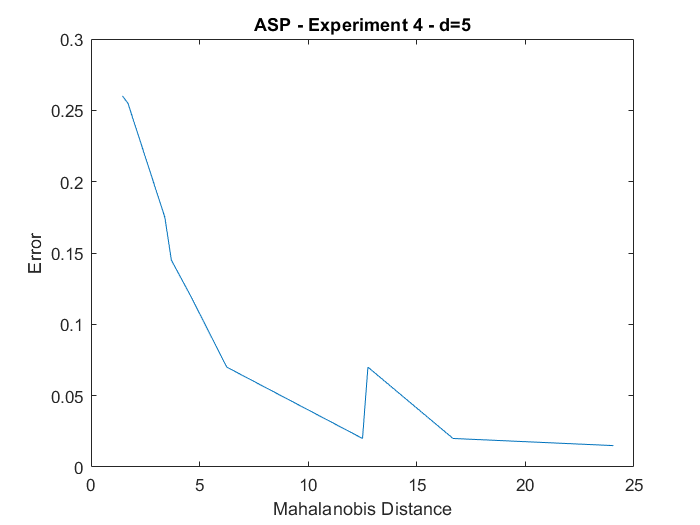
\includegraphics[width=.9\linewidth]{./code/Exp4-results/MahalError_d5_s10.png}
	\caption{Experiment 4 Results}
	\label{fig:exp4}
\end{figure}

    \section{Experiment :}
write a description of the experiment

write a prediction about the outcomes based off theory

\subsection{Results}

results

graphs
\subsection{Discussion}

    \section{Experiment :}
write a description of the experiment

write a prediction about the outcomes based off theory

\subsection{Results}

results

graphs
\subsection{Discussion}

    \section{Conclusions}

All in all 5 out of the 6 stipulated experiments were completed and recorded as above. Primarily the learnings gained through these experiments conclude that the critical features to error probability reduction in pattern recognition and classification algorithms are ensuring an appropriate training data size which contains inside it the right characteristics around the covariance in the classes. Combined with the learnings from the first assignment in this course, it can be assessed that an accurate fit to data models is critical to ensuring accurate classification and that over-fitting or under-fitting can easily be experienced as optimal data sets are rarely realistic in practical applications. The randomized nature of a number of these experiments aided in reaching this conclusion.\\

It's also noted that different classifiers would have different strengths and weaknesses, as seen in utilizing the benefits of the k-Nearest Neighbour classifier to overcome the lack of training data and still improving the performance when compared to the Gaussian classifier used in most of the experiments here.


%    %\bibliographystyle{plain}
%\bibliographystyle{apalike}
%\bibliographystyle{apa}
%\bibliographystyle{natbib}
%\bibliographystyle{vancouver}
%\bibliographystyle{acfrplainnat}
%\bibliographystyle{apalikeAkkaNat}
%\bibliographystyle{ieeetr}
\bibliographystyle{IEEEtran}	%cite order
\newpage
\flushleft
%\bibliographystyle{agsm} %alphabetically organised
\bibliography{A1_VS_6562233,MScDissert-2019-04-21a,OtherSources}

    \newpage
\flushleft
\appendix
\section{Appendix A: Source Code}
\label{App:AppendixA}

\subsection{Experiment 1}
	\lstinputlisting[language=Matlab, caption= Matlab Code developed to simulate experiment 1.]{./code/asp_exp1.m}\label{code:1}

\subsection{Plot 2 Classes}
	\lstinputlisting[language=Matlab, caption= Matlab Code developed to help plot classes in order to visualize the process. Predominantly used in Experiment 1.to simulate experiment 1.]{./code/plot2Classes.m}\label{code:plot}

\subsection{Experiment 2}
	\lstinputlisting[language=Matlab, caption= Matlab Code developed to simulate experiment 2.]{./code/asp_exp2.m}\label{code:2}
	

\subsection{Experiment 3}
	\lstinputlisting[language=Matlab, caption= Matlab Code developed to simulate experiment 3.]{./code/asp_exp3.m}\label{code:3}

\subsection{Experiment 4}
	\lstinputlisting[language=Matlab, caption= Matlab Code developed to simulate experiment 4.]{./code/asp_exp4.m}\label{code:4}


\subsection{Experiment 5}
	\lstinputlisting[language=Matlab, caption= Matlab Code developed to simulate experiment 5.]{./code/asp_exp5.m}\label{code:5}


\subsection{Experiment 6}
	\lstinputlisting[language=Matlab, caption= Matlab Code developed to simulate experiment 6.]{./code/asp_exp6.m}\label{code:6}

\end{document}

